
% This work is licensed under the Creative Commons Attribution-Share Alike 2.0 France License.
% To view a copy of this license, visit http://creativecommons.org/licenses/by-sa/2.0/fr/legalcode
% or send a letter to Creative Commons, 171 Second Street, Suite 300, San Francisco, California, 94105, USA.


\chapter{Tortues et autres choses lentes\label{chap:tortue1}}
\section{Un reptile plus lent que Python}
Il y a certaines similarités entre les tortues du monde réel et une tortue Python.
Dans le monde réel, une tortue   est un reptile, parfois vert, qui se déplace très lentement et porte sa maison sur le dos. Dans le monde de Python, une tortue est une petite flèche noire qui se déplace lentement dans une fenêtre. Néanmoins il n'est nulle part fait mention d'une maison.\\

En fait, considérant le fait que la tortue Python laisse une trace derrière elle dans la fenêtre, cela en fait moins une tortue qu'un petit escargot ou une limace. Néanmoins, je suppose qu'un module appelé « limace »  n'aurait pas été très attirant. C'est pour cela qu'il était plus sensé de garder les tortues. Il suffit d'imaginer une tortue qui transporterait quelques feutres et qui dessinerait en avançant.\\

Dans un passé lointain et sombre il y avait un simple langage de programmation appelé Logo. Logo était utilisé pour contrôler une tortue robot (appelé Irving). Au cours du temps la tortue a évolué depuis un robot qui pouvait se déplacer sur le sol à une petite flèche qui peut se déplacer sur l'écran.\\

\emph{Ce qui revient à montrer que les choses ne s'améliorent pas tout le temps avec les avancés de la technologie. Une petite tortue robot aurait été nettement plus drôle.}\\

\section{À la recherche de la tortue perdue}

Le module « \texttt{turtle\footnote{Le mot \emph{turtle} signifie tortue en anglais et semble venir du français.}} » de Python est juste un petit peu comme la tortue Logo.
Nous verrons plus tard ce qu'est un module, mais 
pour le moment pensez juste que c'est quelque chose.

Néanmoins, Python a de nombreuses autres capacités que Logo. Le module « \texttt{turtle} » est une manière pratique 
 d'apprendre comment les ordinateurs tracent des images sur votre écran.\\

Bon commençons et voyons juste comment cela fonctionne. La première étape est de dire à Python que nous voulons utiliser « \texttt{turtle} » en important le module:

\begin{figure}[ht]
\begin{minipage}{0.4\linewidth}
\scalefont{1.1}
La gestion des fenêtres de Windows, différente de celle des autres systèmes d'exploitation, empêche de laisser le shell Python et la fenêtre « \texttt{turtle} » se recouvrir sans dysfonctionnement. En effet, si le shell Python et la fenêtre « \texttt{turtle} » se recouvrent une seule fenêtre verra son contenu mis à jour. Pour contourner ce problème, vous pouvez utiliser la ligne de commande Python ou réduire la largeur de la fenêtre du shell Python.\\

Vous pouvez voir sur la figure \ref{fig:shellami} le shell Python dont la largeur a été réduite de manière à empêcher le recouvrement.\\

Si le shell n'est pas assez réduit et que la fenêtre « \texttt{turtle} » et le shell sont superposées, il suffit de les déplacer ou de les redimensionner.
\end{minipage}
\hspace{0.5cm}
\begin{minipage}{0.5\linewidth}
\centering
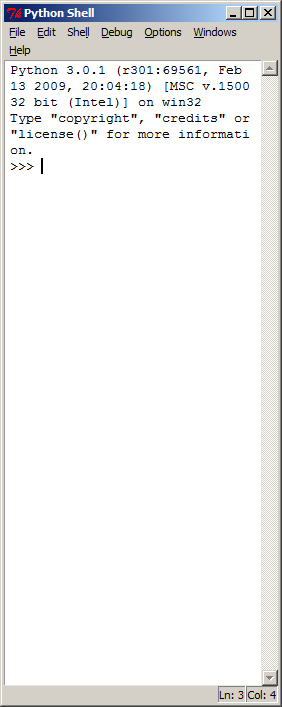
\includegraphics[scale=0.5]{images/shell_pour_turtle.png}
\caption{Shell Python redimensionné pour utiliser turtle}
\label{fig:shellami}
\end{minipage}
\end{figure}

Pour importer le module turtle faites:

\begin{Verbatim}[frame=single,rulecolor=\color{mbleu}, label=à taper]
>>> import turtle
\end{Verbatim}

Puis nous avons besoin d'afficher une feuille pour dessiner. Cette feuille est appelée en informatique zone de dessin. Cette zone de dessin est comme la toile qu'un artiste utilise pour peindre. Dans notre cas c'est juste un espace blanc pour dessiner:

\begin{Verbatim}[frame=single,rulecolor=\color{mbleu}, label=à taper]
>>> tortue = turtle.Pen()
\end{Verbatim}

Attention Python fait la différence entre les minuscules et les capitales\footnote{On dit qu'il est sensible à la casse.}, il convient d'écrire « \texttt{Pen\footnote{Le mot \emph{pen} signifie stylo, du vieux français \emph{penne} lui même du latin tardif \emph{penna} signifiant plume.
}} »  et non pas « \texttt{pen} ». Si vous vous êtes trompés retapez juste: « \texttt{tortue = turtle.Pen()} ».


Quand nous voulons quitter « \texttt{turtle} » il est conseillé de fermer au préalable la zone de dessin en faisant « \texttt{turtle.bye()} ».

\begin{Verbatim}[frame=single,rulecolor=\color{mbleu}, label=à taper]
>>> turtle.Pen()
\end{Verbatim}


Dans \verb+tortue = turtle.Pen()+ nous appelons une fonction particulière (Pen) du module turtle qui crée automatiquement une zone de dessin dans laquelle nous pouvons écrire et nous faisons pointer une variable vers le résultat de cette fonction de manière à pouvoir dessiner.

Une fonction est un bout de code réutilisable (à nouveau nous étudierons  les fonctions plus tard) qui fait quelque chose qu'il est utile de faire plusieurs fois. Dans notre cas la fonction « \texttt{Pen} » retourne un objet qui 
représente notre tortue (enfin notre flèche en forme de tortue). Nous associons cet objet à la variable « \texttt{tortue} ».

Quand nous tapons le code dans la console Python, nous voyons une zone blanche apparaître (la zone de dessin dite \emph{canvas\footnote{Le mot \emph{canvas} signifie toile en anglais du français canevas.}} en programmation) qui ressemble à la figure \ref{fig:turtledebut}

\begin{figure}[ht!]
\centering
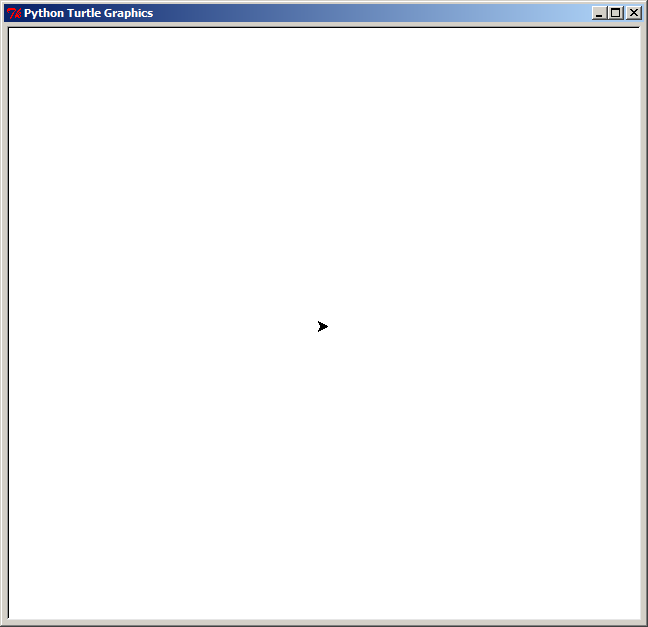
\includegraphics[scale=0.4]{images/turtle_debut.png}
\caption{Une flèche représente la tortue}
\label{fig:turtledebut}
\end{figure}

\emph{Oui la petite flèche au milieu de l'écran est notre tortue. Et non, elle ne ressemble pas vraiment à une tortue.}\\

La \emph{Fausse Bonne Idée} serait de faire :

\begin{Verbatim}[frame=single,rulecolor=\color{red}, label=erreur]
>>> turtle.Pen()
\end{Verbatim}

La zone de dessin serait créée mais sans étiquette pour identifier le stylo, nous ne pourrions pas dessiner dessus.\\


Vous pouvez envoyer des instructions à la tortue, en utilisant des fonctions sur cet objet que nous venons de créer en appelant « \texttt{turtle.Pen} ». Comme nous avons assigné cet objet à la variable tortue, nous utilisons « \texttt{tortue} » pour envoyer des instructions. Une instruction de notre tortue est « \texttt{forward\footnote{Le mot \emph{forward} vers l'avant du vieil anglais foreweard,  \emph{fore} (avant) + \emph{-weard -ward} (suffixe de mouvement).}} ».

L'instruction « \texttt{forward} » dit à notre tortue d'avancer vers l'avant quelque soit la direction vers laquelle elle pointe. Disons à la tortue de bouger vers l'avant de 50 \emph{pixels} (nous allons parler des pixels dans une minute):

\begin{Verbatim}[frame=single,rulecolor=\color{mbleu}, label=à taper]
>>> tortue.forward(50)
\end{Verbatim}

Vous devriez obtenir quelque chose qui ressemble à la figure \ref{fig:50px}.

\begin{figure}[!ht]
\centering
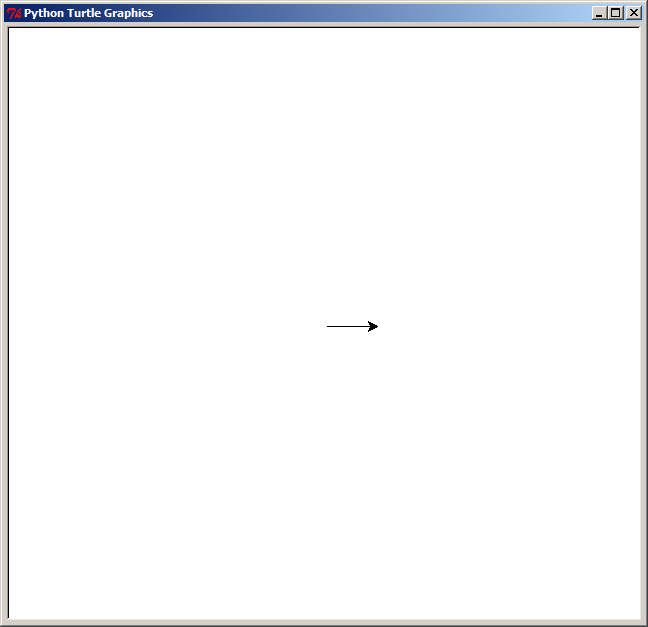
\includegraphics[scale=0.4]{images/50px.png}
\caption{La tortue dessine une ligne}
\label{fig:50px}
\end{figure}

De son point de vue, la tortue a avancé de cinquante pas. Du nôtre, elle s'est déplacée  de 50 pixels.\\


\emph{Bon qu'est-ce que qu'un pixel?}\\

Un pixel est un point sur l'écran. Quand vous regardez l'écran de votre ordinateur tout est fait de petits points (approximativement) carrés. Les programmes que vous utilisez, et les jeux auxquels vous jouez sur l'ordinateur ou votre console, sont faits d'une multitude de différents points colorés arrangés sur l'écran. En fait si vous regardez l'écran avec une loupe vous devriez être capable de voir de quoi sont faits ces points. Ainsi si nous zoomons dans la zone de dessin au niveau de la ligne qui vient d'être tracée par la tortue, nous pouvons voir que la flèche qui représente la tortue est aussi un paquet de points carrés, comme vous pouvez le voir sur la figure \ref{fig:points}.

\begin{figure}[!ht]
\centering
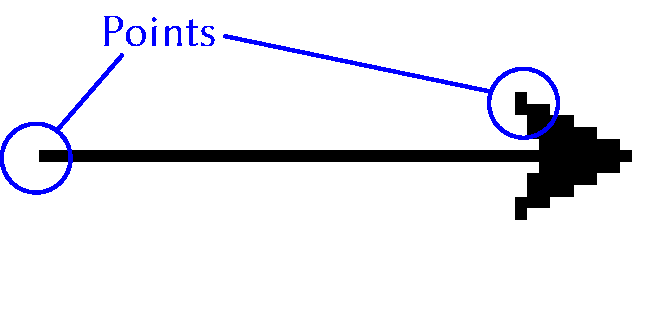
\includegraphics[scale=1]{images/points.pdf}
\caption{Zoom sur la tortue}
\label{fig:points}
\end{figure}

Nous parlerons plus de ces points, ou pixels, dans un prochain chapitre.
Maintenant nous allons dire à la tortue de tourner à gauche ou à droite:

\begin{Verbatim}[frame=single,rulecolor=\color{mbleu}, label=à taper]
>>> tortue.left(90)
\end{Verbatim}

L'instruction « \texttt{left(90)\footnote{Le mot \emph{left} signifie gauche en anglais, du vieil allemand \emph{lucht} (gauche).}} »  dit à la tortue de tourner vers la gauche de 90 degrés (souvent notés °). Vous n'avez peut-être pas encore appris ce que sont les degrés à l'école mais la manière la plus simple de se les représenter est qu'ils sont un peu comme les divisions d'une montre (voir la figure \ref{fig:clock}).
\begin{figure}[H]
\centering
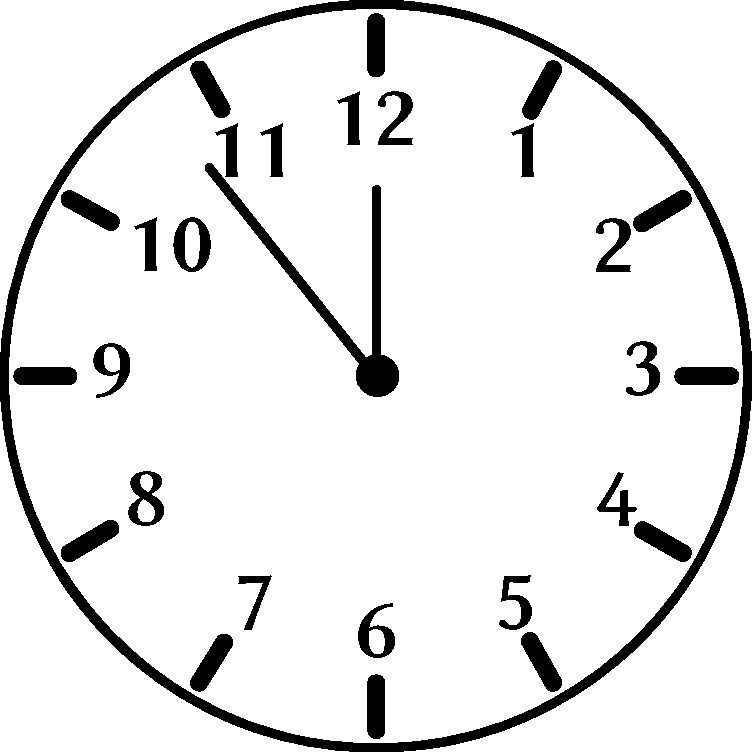
\includegraphics[scale=0.5]{images/clock.pdf}
\caption{Le cadran d'une montre et ses divisions}
\label{fig:clock}
\end{figure}

Contrairement à la montre et à ses 12 divisions (ou 60 si vous comptez les minutes plutôt que les heures), il y faut 360 degrés pour faire un tour complet. Ainsi vous comptez 360 divisions sur l'horloge, vous avez 90 où est normalement 3, 180 là où est normalement 6 et 270 où sont normalement 9. Zéro et 360 seraient en haut au départ où normalement est 12. La figure \ref{fig:degres} vous montre les degrés sur une horloge.
\begin{figure}[H]
\centering
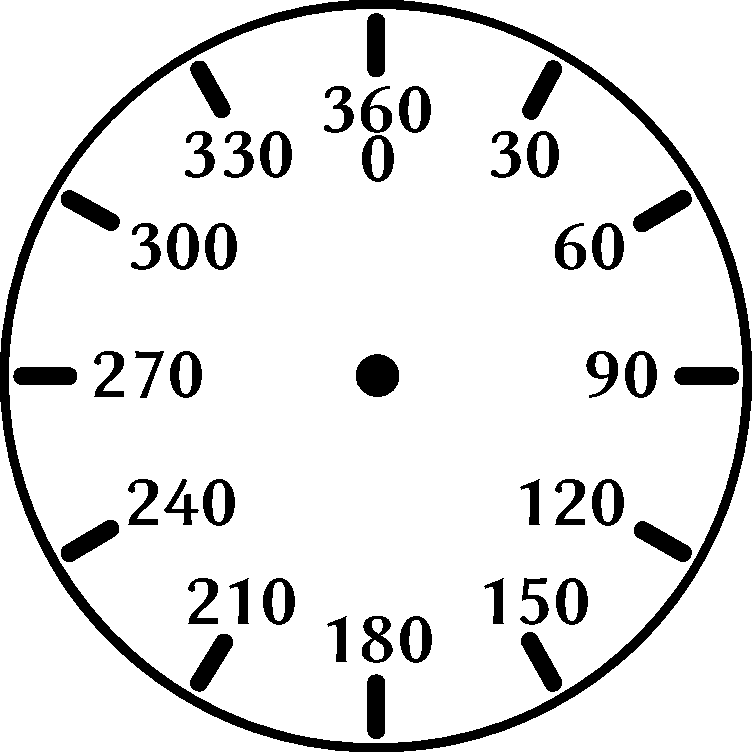
\includegraphics[scale=0.5]{images/degres.pdf}
\caption{Les degrés}
\label{fig:degres}
\end{figure}

Ainsi que veulent vraiment dire « \texttt{left(90)} »  ?\\

Si vous êtes debout et face à une direction, pointez un bras directement dans la continuité de votre épaule, voilà c'est 90 degrés de la direction qui vous fait face (c'est un angle droit). Si vous pointez le bras gauche c'est 90 degrés vers la gauche. Si vous pointez le bras droit c'est 90 degrés vers la droite. Quand la tortue Python tourne vers la gauche, elle met son nez sur un point puis pivote son corps pour pointer vers la nouvelle direction (comme si vous aviez tourné votre corps de manière à faire face vers où le bras pointait).\\

Ainsi suite à « \texttt{tortue.left(90)} »  la tortue-flèche pointe vers le haut, comme montré dans la figure \ref{fig:90l}.
\begin{figure}[!ht]
\centering
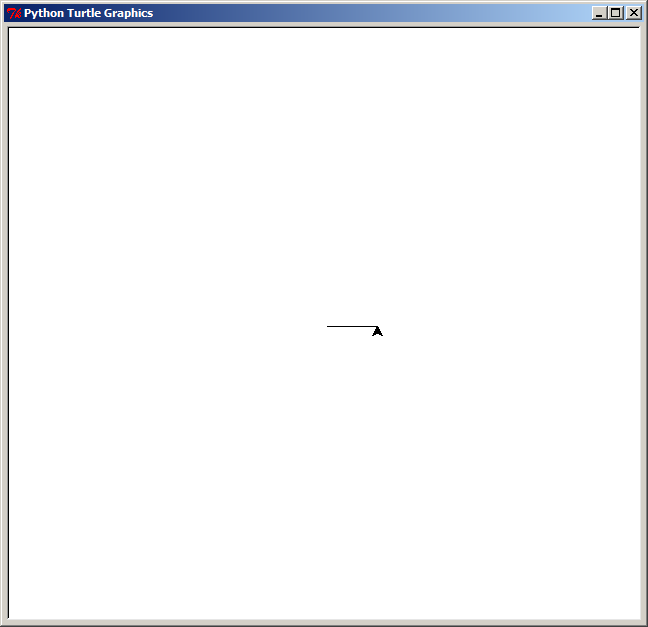
\includegraphics[scale=0.3]{images/90l.png}
\caption{Tortue après avoir tourné de 90°}
\label{fig:90l}
\end{figure}

Recommençons à nouveau quelques fois, en utilisant l'historique:

\begin{Verbatim}[frame=single,rulecolor=\color{mbleu}, label=à taper]
>>> tortue.forward(50)
>>> tortue.left(90)
>>> tortue.forward(50)
>>> tortue.left(90)
>>> tortue.forward(50)
>>> tortue.left(90)
\end{Verbatim}

Notre tortue a dessiné un carré et pointe maintenant dans la même direction et au même endroit que là où elle avait commencé (voir figure \ref{fig:tcar}).
\begin{figure}[!ht]
\centering
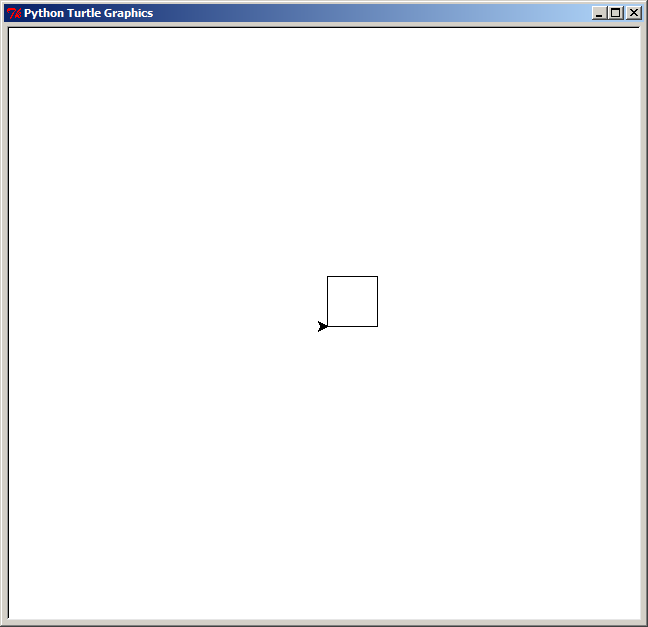
\includegraphics[scale=0.3]{images/tcar.png}
\caption{Tortue après un carré}
\label{fig:tcar}
\end{figure}

Nous pouvons effacer ce qu'il y a sur la zone de dessin en utilisant « \texttt{clear()} » (effacer en anglais).

Il  existe quelques autres fonctions que vous pouvez utiliser: 
\begin{itemize}
\item « \texttt{right()} »\footnote{droite en anglais} qui tourne la tortue vers la droite;
\item « \texttt{reset()} »\footnote{remise à zéro en anglais} qui elle aussi efface l'écran mais replace automatique la tortue à sa position initiale;
\item « \texttt{backward()} »\footnote{vers l'arrière en anglais} qui fait reculer la tortue;
\item « \texttt{up()} »\footnote{vers le haut} qui dit à la tortue de ne plus dessiner (qui soulève le stylo);
\item « \texttt{down()} »\footnote{vers le bas} qui dit à la tortue de dessiner à nouveau.
\end{itemize}
 Vous pouvez utiliser ces fonctions de la même manière que vous avez utilisé les autres:
 
\begin{Verbatim}[frame=single,rulecolor=\color{mbleu}, label=à taper]
>>> tortue.reset()
>>> tortue.backward(100)
>>> tortue.right(90)
>>> tortue.forward(100)
>>> tortue.up()
>>> tortue.forward(100)
>>> tortue.down()
>>> tortue.forward(100)
\end{Verbatim}

Nous reviendrons au module « \texttt{turtle} »  bientôt.

\section{À vous de jouer}\label{PRATIQUE:TORTUES}
Dans ce chapitre nous avons vu comment utiliser la tortue pour dessiner de simples lignes, la faire tourner à gauche et à droite. Nous avons vu que la tortue utilise des degrés pour tourner, un peu comme des minutes sur un horloge.

Vous trouverez des pistes de réponses dans la \autoref{REPONSES:TORTUES}.
\subsection*{Exercice 1}
Créez une zone de dessin en utilisant la fonction Pen() de « \texttt{turtle} » et dessinez un rectangle.
\subsection*{Exercice 2}
Créez une autre zone de dessin en utilisant la fonction Pen() de « \texttt{turtle} » et dessinez un triangle.
 \vfill
\begin{center}
 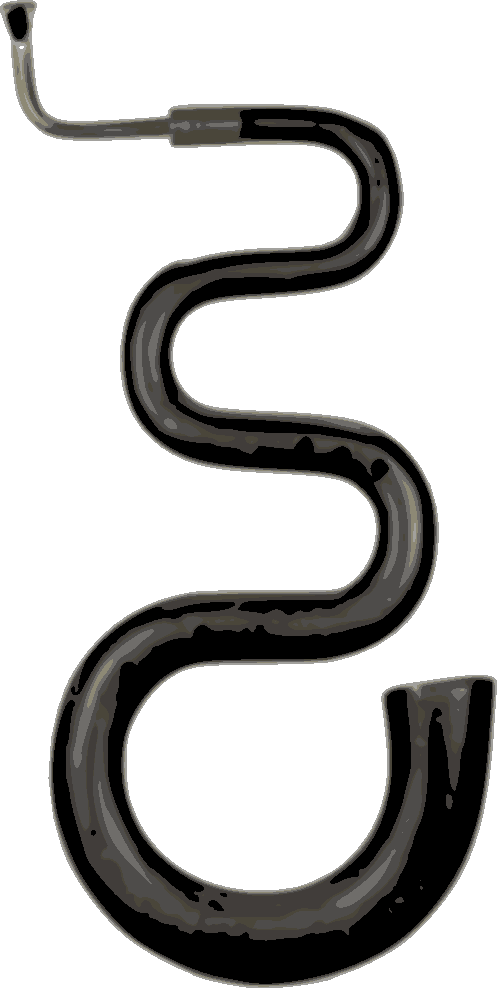
\includegraphics[width=5cm]{images/sem.pdf}
\end{center}
 \vfill

\clearemptydoublepage
